\documentclass{article}
\usepackage[T2A]{fontenc}
\usepackage[utf8]{inputenc}
\usepackage[russian]{babel}
\usepackage{textcomp}
\usepackage{color}
\usepackage{xspace}
\usepackage{multirow}
\usepackage{amsmath,amsfonts,amsthm,amssymb,amsbsy,amstext,amscd,amsxtra,multicol}
\usepackage{indentfirst}
\usepackage{verbatim}
\usepackage[left=2cm, right=2cm, top=2cm, bottom=2cm, bindingoffset=0cm]{geometry}
\usepackage[pdf]{graphviz}
\usepackage{morewrites}
\usepackage{multicol}
\usepackage{graphicx}
\graphicspath{ {./} }

\usepackage{hyperref}
\hypersetup{
    colorlinks=true,
    linkcolor=blue,
    filecolor=magenta,      
    urlcolor=cyan,
    pdfpagemode=FullScreen,
}

\urlstyle{same}

\usepackage{xpatch}
\makeatletter
\newcommand*{\addFileDependency}[1]{% argument=file name and extension
  \typeout{(#1)}
  \@addtofilelist{#1}
  \IfFileExists{#1}{}{\typeout{No file #1.}}
}
\makeatother
\xpretocmd{\digraph}{\addFileDependency{#2.dot}}{}{}



\begin{document}
    \vbox{%
        \hfill%
        \vbox{%
            \hbox{\large Выполнил студент группы А-05-19 \par}%
            \hbox{\large Трофимов Илья Сергеевич \par}%
            \hbox{\large 27 мая 2022 г.\par}%
        }%
    } 
    
    \begin{center}
        {\Large \textbf{Домашняя работа №3}\par}
        \includegraphics[scale=0.09]{wordart.png}
    \end{center}
    
    \textbf{ЗАДАНИЕ 1. Операции с числами}\\
    Реализуйте машины Тьюринга, которые позволяют выполнять следующие операции:
    \begin{enumerate}
        \item \textbf{Сложение двух унарных чисел}\\
        Машина Тьюринга принимает две последовательности единиц, разделённых плюсом (например, 1111+11), после выполнения алгоритма машина установит каретку на начало результрующего числа. Машина будет удалять первую единицу  и заменять знак + между числами на единицу, тем самым 'склеивая'  аргументы. составить таблицу переходов (использую нотацию из курса мат. логики):
        \begin{center}
            \begin{tabular}{ |c||c|c|c| }
            \hline
            состояние & 1 & + & \varepsilon \\ 
            \hline
            \hline
            first & toPlus, \varepsilon, R & done, \varepsilon, R & \\\hline
            toPlus & R & toStart, 1, L & \\\hline    
            toStart & L &  & done, R \\\hline   
            done &  &  & H \\\hline
            \end{tabular}
        \end{center}
        Код для реализации машины Тьюринга доступен по
        \href{https://github.com/NRU-MPEI-IMAI/tm-and-qc-IliaTrofimov/blob/main/1_1.yaml}{этой ссылке}.
        
        \item \textbf{Умножение унарных чисел}\\
        Для того, чтобы составить машину Тьюринга определим умножение следующим образом:
        \begin{center}
             mult(0, \(b\)) = 0\\
             mult(\(a\),  \(b\)) =  \(b\) + mult(\(a-1\), \(b\))
        \end{center}
        Машина Тьюринга принимает две последовательности единиц, разделённых знаком умножения (например, 1111*11), после выполнения алгоритма машина установит каретку на начало результрующего числа. Суть алгоритма заключается в последовательном уменьшении \(a\) и копировании \(b\) на каждом шаге. Составим таблицу переходов:
        \begin{center}
            \begin{tabular}{ |c||c|c|c| }
            \hline
            состояние & 1 & * & \varepsilon \\ 
            \hline
            \hline
            eachA & toB, \varepsilon, R & skip, *, R & \\\hline
            toB & R & eachB, *, R & \\\hline    
            nextA & L & L & eachA, 1,  R \\\hline   
            skip & R &  & H \\\hline
            eachB & sep, \varepsilon, R &  &  nextA, \varepsilon, L\\\hline  
            sep & add, 1, R &  &  R\\\hline  
            add & R &  &  1, sepL, \varepsilon, L\\\hline  
            sepL & L &  &  nextB, \varepsilon,  L\\\hline  
            nextB & L &  &  eachB, 1,  R\\\hline
            \end{tabular}
        \end{center}
        Код для реализации машины Тьюринга доступен по
        \href{https://github.com/NRU-MPEI-IMAI/tm-and-qc-IliaTrofimov/blob/main/1_2.yaml}{этой ссылке}.
    \end{enumerate}
    
    \textbf{ЗАДАНИЕ 2. Операции с языками и символами}\\ 
    Реализуйте машины Тьюринга, которые позволяют выполнять следующие операции:
    \begin{enumerate}
        \item \textbf{Принадлежность к языку \(L=\{0^n1^n2^n\}, n \ge 0\).}\\
        Машина Тьюринга будет принимать слово и в конце совей работы записывать T, если слово принадлежит языку, и F - если не принадлежит.\\
        Будем помечать тройки из символов 0, 1, 2 буквами a, b, c, продвигаясь по слову вперёд. Как только пометим все буквы и достигнем пустого символа, можем считать, что исходное слово принадлежит языку \(L\), если по какой-то причине этого не удалось сделать (например, раньше чем нужно достигли конца или встретили неожиданный символ), то слово не принадлежит языку.\\
        Составим таблицу переходов:
        \begin{center}
            \begin{tabular}{ |c||c|c|c|c|c|c|c| }
            \hline
            состояние & 0 & 1 & 2 & \(a\) & \(b\) & \(c\) &\varepsilon \\ 
            \hline
            \hline
            \(q_0\) & \(q_1aR\) & \(q_{end}FR\) & \(q_{end}FR\) & \(q_{end}FR\) & \(q_{scan}bR\) & \(q_{end}TR\) & \\\hline
            \(q_1\) & \(R\) & \(q_2bR\) &  &  & \(R\) &  & \\\hline
            \(q_2\) & & \(R\) & \(q_{back}cR\) &  &  & \(R\) &  \\\hline
            \(q_{back}\) & \(L\) & \(L\) & & \(q_0aR\) & \(L\) & \(L\) &  \\\hline
            \(q_{scan}\) & \(q_{end}FR\) & \(q_{end}FR\) & \(q_{end}FR\) & \(q_{end}FR\)  & \(R\) & \(R\) & \(q_{end}TR\) \\\hline
            \(q_{end}\) & & & &  &  &  & \(L\) \\\hline
            \end{tabular}
        \end{center}
         Код для реализации машины Тьюринга доступен по
        \href{https://github.com/NRU-MPEI-IMAI/tm-and-qc-IliaTrofimov/blob/main/2_1.yaml}{этой ссылке}.
        
        \item \textbf{Проверка соблюдения правильности скобок в строке}\\
        Пусть машина Тьюринга принимает последовательность скобок и в конце своей работы устанавливает T, если последовательность правильная, F - если неправильная. Будем пользоваться следующим алгоритмом:
        \begin{itemize}
            \item Движемся вправо до появления некоторой закрывающей скобки, пусть ), заменяем её буквой A (другие скобки заменяем другими буквами). 
            \item Теперь возвращаемся назад, пока не найдём соответсвующую открывающую скобку, пропуская все помеченные скобки, если найдём открывающую скобку другого типа или пустой символ (т.е. вернёмся в начало), то слово неправильное.
            \item Нужную открывающую скобку тоже заменяем на A и повоторяем этот процесс.
        \end{itemize}
        Если, выполняя данный процесс, достигли пустого символа (в данном случае конца слова), то слово правильное.\\
        Составим таблицу переходов:
        \begin{center}
            \begin{tabular}{ |c||c|c|c|c|c|c|c|c|c|c| }
            \hline
            состояние & ( & \langle & \} & ) & \rangle &\} & \(A\) & \(B\) & \(C\) &\varepsilon \\ 
            \hline
            \hline
            \(q_{right}\)&\(R\)&\(R\)&\(R\)&\(q_aAR\)&\(q_bBR\)&\(q_cCR\)&\(R\)&\(R\)&\(R\)&\(q_{end}TR\)\\\hline
            \(q_A\)     &\(q_{right}AR\)&\(q_{end}FR\)&\(q_{end}FR\)&&&&\(L\)&\(L\)&\(L\)&\(q_{end}FR\)\\\hline
            \(q_B\)     &\(q_{end}FR\)&\(q_{right}BR\)&\(q_{end}FR\)& & & &\(L\)&\(L\)&\(L\)&\(q_{end}FR\)\\\hline
            \(q_C\)     &\(q_{end}FR\)&\(q_{end}FR\)&\(q_{right}CR\)& & & &\(L\)&\(L\)&\(L\)&\(q_{end}FR\)\\\hline
            \(q_{end}\)  & & & & & & &\(L\)&\(L\)&\(L\)&\(L\)\\\hline 
            \end{tabular}
        \end{center}
         Код для реализации машины Тьюринга доступен по
        \href{https://github.com/NRU-MPEI-IMAI/tm-and-qc-IliaTrofimov/blob/main/2_2.yaml}{этой ссылке}.
        
                \item \textbf{Поиск минимальной строки}\\
        Машина Тьюринга принимает последовательность строк из 0 и 1, разделённых тире (т.к. в turingmachine.io пробелом отмечается пустой символ) и в конце своей работы устаналивает каретку на начало наименьшей строки.\\
        Для нахождения минимальной строки будем помечать по одному символу каждой строки до тех пор пока не дойдём до разделителя-тире. После этого счтиаем, что минимальная строка найдена (она позади). Зачищаем ленту от ненужных строк и возвращаем каретку. Готово.\\
        Составим таблицу переходов:
        \begin{center}
            \begin{tabular}{ |c||с|c|c|c|c|c| }
            \hline
            состояние & 0 & 1 & a & b & - & \varepsilon \\\hline \hline
            mark & next, a, R & next, b, R & R & R & clear, R & reset, L \\\hline
            next & R & R & & & mark, R & back, L \\\hline
            back & L & L & L & L & L & mark, R \\\hline
            clear& \varepsilon,R &  \varepsilon,R & \varepsilon,R &  \varepsilon,R &  \varepsilon,R & return, L \\\hline
            return & & & & & \varepsilon,R & reset, L \\\hline
            reset & 0, L & 1, L & & & done, R & done, R\\\hline
            done & H & H & & & & H \\\hline
            \end{tabular}
        \end{center}
        Код для реализации машины Тьюринга доступен по
        \href{https://github.com/NRU-MPEI-IMAI/tm-and-qc-IliaTrofimov/blob/main/2_3.yaml}{этой ссылке}.
    
    \end{enumerate}
    
        \textbf{ЗАДАНИЕ 3. Квантовые вычисления}\\ 
    Все функции для решений следующих заданий расположены в репозитории по \href{https://github.com/NRU-MPEI-IMAI/tm-and-qc-IliaTrofimov/blob/main/task-3.qs}{этой ссылке}.
    \begin{enumerate}
        \item \textbf{Генерация суперпозиций.}\\
        Дано $N$ кубитов ($1 \le N \le 8$) в нулевом состоянии $\Ket{0\dots0}$. Также дана некоторая последовательность битов, которое задаёт ненулевое базисное состояние размера $N$. Задача получить суперпозицию нулевого состояния и заданного.\\
        Решение на Q\#: \begin{verbatim}
operation Set (desired: Result, q1: Qubit) : () {
    body {
        let current = M(q1);
        if (desired != current) { 
            X(q1);
        }
    }
}

operation Super(qs: Qubit[], bits: Bool[]) : () {
    body {   
        // Предварительно зануляем кубиты
        for (q in qs) {
            Set(Zero, q);
        }
        
        H(qs[0]);
        for (i in 1..Length(qs) - 1) {
            if (bits[i]) {
                CNOT(qs[0], qs[i]); 
            } 
        }                  
    }
}
        \end{verbatim}
        Схема для случая \(|0 0 0 0 \rangle\), \(|1 0 1 1 \rangle\): 
        \begin{center}
            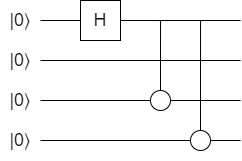
\includegraphics[scale=0.5]{1.png}
        \end{center}
        
        \item \textbf{Различие состояний 1.}\\
        Дано $N$ кубитов ($1 \le N \le 8$), которые могут быть в одном из двух состояний:
        $$\Ket{GHZ} = \frac{1}{\sqrt2}(\Ket{0\dots0} +\Ket{1\dots1})$$
        $$\Ket{W} = \frac{1}{\sqrt N}(\Ket{10\dots00}+\Ket{01\dots00} + \dots +\Ket{00\dots01})$$
        Требуется выполнить необходимые преобразования, чтобы точно различить эти два состояния. Возвращать $0$, если первое состояние и 1, если второе.\\
        Решение на Q\#: \begin{verbatim}
operation Determine1(qs: Qubit[]) : Int {
    body {   
        mutable ones = 0;
        for (q in qs) {
            if (M(q) == One) { 
                set ones = ones + 1; 
            }
        }
        if (ones == 1) {
            return 1;
        } 
        else {
            return 0;
        }                
    }
}
        \end{verbatim}
        
        \item \textbf{Различие состояний 2.}\\
        Дано $2$ кубита, которые могут быть в одном из двух состояний:
        $$\Ket{S_0} = \frac{1}{2}(\Ket{00} + \Ket{01} + \Ket{10} + \Ket{11}), \ \Ket{S_1} = \frac{1}{2}(\Ket{00} - \Ket{01} + \Ket{10} - \Ket{11}),$$
        $$\Ket{S_2} = \frac{1}{2}(\Ket{00} + \Ket{01} - \Ket{10} - \Ket{11}), \ \Ket{S_3} = \frac{1}{2}(\Ket{00} - \Ket{01} - \Ket{10} + \Ket{11}$$
        Требуется выполнить необходимые преобразования, чтобы точно различить эти четыре состояния. Возвращать требуется индекс состояния (от $0$ до $3$).\\
        Решение на Q\#: 
        \begin{verbatim}
 operation Determine2(q1: Qubit, q2: Qubit) : Int {
    if (M(q1) == Zero) {
        if (M(q2) == Zero) { return 0; } 
        else { return 1; }
    }
    else {
        if (M(q2) == Zero) { return 2; } 
        else { return 3; }
    }
}
    \end{verbatim}
    
    \item \textbf{Написание оракула.}\\
    Требуется реализовать квантовый оракул на $N$ кубитах ($1 \le N \le 8$), который реализует следующую функцию: $f(\pmb{x}) = (\pmb{b}\pmb{x}) \mod 2$, где  $\pmb{b} \in \{0,1\}^N$ вектор битов и  $\pmb{x}$ вектор кубитов. Выход функции записать в кубит $\pmb{y}$. Количество кубитов $N$ ($1 \le N \le 8$).\\
    Решение на Q\#: 
    \begin{verbatim}
operation Oracle(x : Qubit[], y : Qubit, b : Int[]) : () {
    body {
        for (i in 0..Length(x) - 1) {
            if (b[i] == 1) {
                CNOT(x[i], y);
            } 
            else {
                Set(Zero, y);
            }
        }
    }
} 
    \end{verbatim}
    \end{enumerate}
    
    Все функции для решений следующих заданий расположены в репозитории по \href{https://github.com/NRU-MPEI-IMAI/tm-and-qc-IliaTrofimov/blob/main/task-3.qs}{этой ссылке}.
    
\end{document}
